\documentclass{report}

\usepackage{ugentstyle}
\usepackage{listings}

\begin{document}
	\maketitle{Beveiliging van netwerken en computers}
	\tableofcontents
	
	\chapter{Routing + DNS}
	De bedoeling van dit labo is een netwerkconfiguratie op te stellen en een DNS-server op te zetten die je in latere labo's nog zal gebruiken. Zorg er dus voor dat je de configuratie waar mogelijk persistent maakt, en eventueel de nodige commando's in scripts opneemt zodat je tijdens volgende labo's de opstelling snel kan herstellen.  Vooraleer aan de instellingen van de (fysieke) labotoestellen iets te veranderen maak je een volledige backup van de \textbackslash etc directory (tar -cvjf \textbackslash root \textbackslash backup\_etc.tar.bz2 \textbackslash etc).
	Editeer geen enkel configuratiebestand zonder er eerst een kopie van te maken!
	
	Voor dit labo werken we met groepjes van twee studenten. Iedere groep zal zich ontfermen over één DNS-domein dat vier hosts omvat (twee fysieke toestellen en twee virtuele machines). Ieder fysiek toestel zal dus als host fungeren voor één virtuele machine. Figuur \ref{fig:opstelling} geeft een algemeen overzicht van de opstelling voor één groep.
	\begin{figure}
		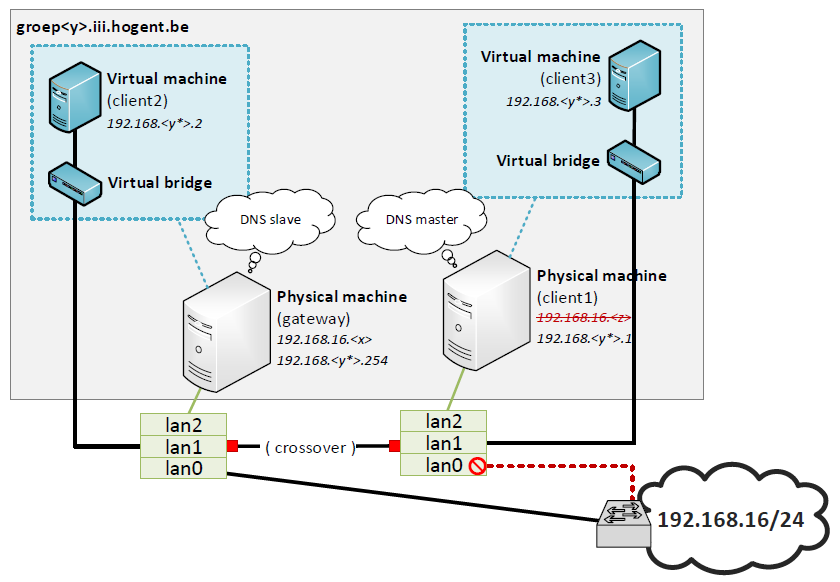
\includegraphics[width=\textwidth]{opstelling}
		\caption{Opstelling}
		\label{fig:opstelling}
	\end{figure}
	Voor de uitwerking van dit labo wordt de groep op figuur \ref{fig:groep} gebruikt.
	\begin{figure}
		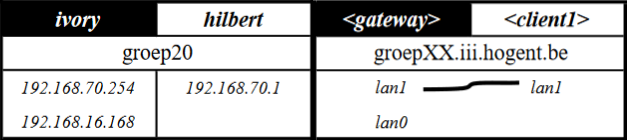
\includegraphics[width=\textwidth]{groep}
		\caption{Een groep}
		\label{fig:groep}
	\end{figure}
\section{Routing}
 Voor elke groep bestaat de opstelling uit vier verschillende hosts:
\begin{itemize}
	\item \textbf{gateway}: deze verbindt het interne netwerk van jouw groep met het HoGent netwerk via onze gateway 192.168.16.8. Dit toestel is via een crosskabel (lan1) verbonden met de tweede fysieke machine (client1).
	\item \textbf{client1}: deze is via een crosskabel (lan1) verbonden met de gateway. Merk op dat dit toestel niet rechtstreeks verbonden is met het HoGent netwerk!
	\item \textbf{client2}: dit is een virtuele machine die draait op de gateway. Deze virtuele machine is via een virtuele bridge verbonden met het interne netwerk (lan1) van de gateway.
	\item \textbf{client3}: dit is een virtuele machine die draait op client1. Deze virtuele machine is via een virtuele bridge verbonden met het interne netwerk (lan1) van client1.
	
\end{itemize}
\subsection{Configuratie IP-adressen}
Voor de netwerkconfiguratie maak je overal gebruik van statische IP-adressen (ook voor lan0 op de gateway). Om te testen kan je eerst gebruikmaken van het \textit{ip} commando, maar uiteindelijk is het eenvoudigst om een configuratiebestand te voorzien per interface. De configuratiebestanden vind je bij Fedora terug in de folder \texttt{/etc/sysconfig/network-scripts/}. 
\begin{itemize}
	\item \textbf{Gateway}: \begin{itemize}
								\item \texttt{ifcfg-lan0}:
									  		\begin{lstlisting}
DEVICE=lan0
BOOTPROTO=none
ONBOOT=yes
NETMASK=255.255.255.0
IPADDR=192.168.16.168
GATEWAY=192.168.16.8
											\end{lstlisting}
								\item \texttt{ifcfg-lan1}:
\begin{lstlisting}
DEVICE=lan0
BOOTPROTO=none
ONBOOT=yes
NETMASK=255.255.255.0
IPADDR=192.168.70.254
\end{lstlisting}											
							\end{itemize}
	\item \textbf{Client1}: 
	\begin{itemize}
		\item \texttt{ifcfg-lan1}:
		\begin{lstlisting}
DEVICE=lan1
BOOTPROTO=none
ONBOOT=yes
NETMASK=255.255.255.0
IPADDR=192.168.70.1
GATEWAY=192.168.70.254
		\end{lstlisting}										
	\end{itemize}

	\item \textbf{Client2}: 
\begin{itemize}
	\item \texttt{ifcfg-enp0s3}:
	\begin{lstlisting}
DEVICE=enp0s3
BOOTPROTO=none
ONBOOT=yes
NETMASK=255.255.255.0
IPADDR=192.168.70.2
GATEWAY=192.168.70.254
	\end{lstlisting}										
\end{itemize}

	\item \textbf{Client3}: 
\begin{itemize}
	\item \texttt{ifcfg-enp0s3}:
	\begin{lstlisting}
DEVICE=enp0s3
BOOTPROTO=none
ONBOOT=yes
NETMASK=255.255.255.0
IPADDR=192.168.70.3
GATEWAY=192.168.70.254
	\end{lstlisting}										
\end{itemize}

\end{itemize}

\subsection{OSPF}

Op de gateway gebruik je OSPF om de route naar jouw subnet te multicasten. Als router-software maak je gebruik van quagga en twee zelfgemaakte configuratiebestanden zebra.conf en ospfd.conf die je in de directory \texttt{/etc/quagga} plaatst. Aangezien iedere gateway rechtstreeks verbonden is met het 192.168.16.0/24 netwerk laten we dit overeenstemmen met area 0. Het is dus niet nodig om bijkomende areas in het leven te roepen!
Ken aan je interfaces geen IP-adressen toe via quagga maar doe dit dus op de traditionele manier met het commando ip of via ifcfg-files.
Vergeet niet om routing actief te zetten op de nodige hosts.
Om te testen of je configuratie werkt, moet je zowel de zebra daemon als de ospfd daemon starten. 

\begin{itemize}
	\item \textbf{zebra.conf}:
		\begin{lstlisting}
hostname ivory
password pass
enable password pass
log stdout
!
interface lan0
!
interface lan1
!
		\end{lstlisting}
	\item \textbf{ospfd.conf}:
		\begin{lstlisting}
hostname ivory
password pass
enable password pass
log stdout
!
interface lan0
!
interface lan1
!
router ospf
	redistribute connected
	network 192.168.16.0/24 area 0.0.0.0
!
\end{lstlisting}

\end{itemize}
Voeg \texttt{net.ipv4.ip\_forward = 1} toe aan het bestand \texttt{/etc/sysctl.conf}. 
Voer nu het commando \texttt{systemctl status/restart/enable zebra/ospfd} uit. \textit{Restart} zal de daemon herstarten en \textit{enable} geeft aan dat de daemon bij de bootprocedure moet opgestart worden. Met \textit{status} kan nagegaan worden of dat de configuratie correct verlopen is.
\section{DNS}
Binnen de opstelling configureer je ook twee DNS-servers die verantwoordelijk zijn voor het subdomein van de groep (groep20.iii.hogent.be). \textbf{client1} doet dienst als primaire (master) DNS-server, de \textbf{gateway} als secundaire (slave) DNS-server. Binnen je domein voorzie je zowel een forward als een reverse DNS lookup zone. Alle aanvragen die niet voor jouw domein bedoeld zijn stuur je via een \textbf{forwarder} door naar 192.168.16.8. 
\subsection{Configuratie named}
 Wij hebben reeds voor jou een DNS-root-server geconfigureerd. Bijgevolg kunnen alle DNS-aanvragen die geen betrekking hebben op jouw domein doorgestuurd worden naar 192.168.16.8. Dit is ook de default-gateway van de router en moet als dusdanig worden ingesteld. Jouw DNS-server voorziet in de naamgeving voor de vier hosts in het domein. Om voldoende redundantie te hebben, configureer je op de gateway een secundaire nameserver.

Voor DNS maken we gebruik van de BIND/named service die reeds op de fysieke toestellen geïnstalleerd is. De configuratie moet je zelf nog aanpassen of aanmaken. Maak hiervoor gebruik van volgende directories en bestanden:

\begin{itemize}
	\item \texttt{/etc/named.conf}: algemene configuratie BIND/named.
	\item \texttt{/var/named/}: zonebestanden voor jouw domein
\end{itemize}


Om te testen of het configuratiebestand en de zonebestanden correct zijn, kan je respectievelijk gebruikmaken van de \texttt{named-checkconf} en \texttt{named-checkzone} commando's. Eenmaal de configuratie correct is, kan je de named service (her)starten via het systemctl commando.
Voor de virtuele machines gebruik je als hostname de naam van je toestel, gevolgd door 'VM'. De virtuele machine op computer Kronecker zal bv. de naam KroneckerVM hebben.
Voorzie zowel een forward als een reverse DNS lookup zone die de vier hosts bevat en test grondig uit! Aangezien veel services die we tijdens de labo's gebruiken steunen op reverse DNS, is het belangrijk dat deze correct geconfigureerd is. 
\begin{itemize}
	\item \textbf{/etc/named.conf}: 
	\begin{itemize}
		\item client1:
			\begin{lstlisting}
options {
	directory	"/var/named";
	dump-file	"/var/named/data/cache_dump.db";
	statistics-file	"/var/named/data/named_stats.txt";
	memstatistics-file "var/named/data/named_mem_stats.txt";
	allow-query	{ any; };
	recursion yes,
	empty-zones-enable no;
	forwarders { 192.168.16.8; };
};

logging {
	channel default_debug {
		syslog daemon;
		severity dynamic;
	}
};

zone "groep20.iii.hogent.be" IN {
	type master;
	file "groep20.iii.hogent.be";
	allow-transfer { 192.168.70.254; };
};

zone "70.168.192.in-addr.arpa" {
	type master;
	file "70.168.192.in-addr.arpa";
	allow-transfer { 192.168.70.254; };	
};

			\end{lstlisting}
		\item gateway: 
		\begin{lstlisting}
options {
	directory	"/var/named";
	dump-file	"/var/named/data/cache_dump.db";
	statistics-file	"/var/named/data/named_stats.txt";
	memstatistics-file "var/named/data/named_mem_stats.txt";
	allow-query	{ any; };
	recursion yes,
	empty-zones-enable no;
	forwarders { 192.168.16.8; };
};

logging {
	channel default_debug {
		syslog daemon;
		severity dynamic;
	}
};

zone "groep20.iii.hogent.be" IN {
	type slave;
	file "groep20.iii.hogent.be";
	masters { 192.168.70.254; };
};

zone "70.168.192.in-addr.arpa" {
	type slave;
	file "70.168.192.in-addr.arpa";
	masters { 192.168.70.254; };
};
		\end{lstlisting}
	\end{itemize}
	\item \textbf{/var/named/groep20.iii.hogent.be}
	\begin{lstlisting}
$TTL 60
@ IN SOA groep20.iii.hogent.be. bert.desaffel.ugent.be (1 60 1H 60 3H)
  IN NS	 hilbert
  IN NS  ivory
hilbert 	IN	A	192.168.70.1
hilbertVM 	IN	A	192.168.70.3
ivory 		IN	A	192.168.70.254
ivoryVM	 	IN	A	192.168.70.4
	\end{lstlisting}
	\item \textbf{/var/named/70.168.192.in-addr.arpa}
	\begin{lstlisting}
$TTL 60
@   IN SOA 70.168.192 bert.desaffel.ugent.be (1 60 1H 60 3H)
    IN NS hilbert.groep20.iii.hogent.be.	
1   IN PTR hilbert.groep20.iii.hogent.be.
3   IN PTR hilbertVM.groep20.iii.hogent.be.
2   IN PTR ivoryVM.groep20.iii.hogent.be.
254 IN PTR ivory.groep20.iii.hogent.be.
	\end{lstlisting}	
\end{itemize}

\subsection{Clientconfiguratie}
Alle hosts moeten gebruikmaken van de eigen DNS-servers, hiervoor pas je \texttt{/etc/resolv.conf} aan. Voeg aan dit bestand ook een optie toe om de verschillende DNS-aanvragen over beide nameservers te verdelen.
Zorg er voor dat DHCP uitgeschakeld is (BOOTPROTO=none in de ifcfg-files) voor elke netwerkinterface van de host! Indien dit niet het geval is, zal de dhcp-client bij elke herstart de inhoud van het /etc/resolv.conf bestand overschrijven.

Bovendien stel je ook op elk van de 4 clients de juiste hostname in, maak hierbij gebruik van de Fully Qualified Domain Name (FQDN). Om de hostname in te stellen kan je gebruikmaken van onderstaande commando's. 
\begin{lstlisting}
hostnamectl set-hostname --static <name>.groep20.iii.hogent.be
hostnamectl set-hostname --transient <name>.groep20.iii.hogent.be
hostnamectl set-hostname --pretty <name>.groep20.iii.hogent.be
\end{lstlisting}
Op alle vier de toestellen in \texttt{/etc/resolv.conf}:
\begin{lstlisting}
domain groep20.iii.hogent.be
nameserver 192.168.70.1
nameserver 192.168.70.254
options rotate
\end{lstlisting}
\section{Uittesten}
 Vooraleer de opstelling af te breken test je deze grondig uit! Eventueel kan je ook alle machines eens herstarten, om na te gaan of de configuratie volledig persistent is.
	
	Uiteindelijk moet je vanaf elke host alle toestellen binnen het eigen netwerk kunnen bereiken. Dit kan je eenvoudig testen via het ping commando. Bovendien moet je vanaf elke host ook onze gateway (192.168.16.8) kunnen bereiken, alsook alle toestellen van de andere groepen binnen het lokaal. Een ping pakket sturen naar buiten (bv. ping google.be) heeft weinig zin, aangezien de firewall van de HoGent alle ICMP-pakketten blokkeert.
	
	Om je DNS-server te testen kan je gebruikmaken van het dig commando. Test je DNS-servers kritisch uit, en probeer ook of je het domein van je buren kan bereiken. 

\chapter{SSH}
 Voor dit deel maak je gebruik van de virtuele machines die je in het vorige labo hebt aangemaakt. Maak vooraf een zip van de virtuele harde schijf die je na afloop van het labo terugplaatst. Wijzig in geen geval de configuratiebestanden van de fysieke toestellen.

Het aanpassen van de configuratie en het herstarten van de server doe je als root-gebruiker.
Het configureren en uitvoeren van de de client-commando's doe je meestal als een gewone gebruiker (tiwi1, ...), soms als root indien nodig. Maak daarom bij het begin van dit labo 3 extra gebruikers aan op je virtuele machine: tiwi1, tiwi2 en tiwi3 (zelfde wachtwoord als root). 
\begin{lstlisting}
(in de command shell)
adduser tiwi1
passwd tiwi1 
root
adduser tiwi2
passwd tiwi2
root
adduser tiwi3
passwd tiwi3
root
\end{lstlisting}
Om in te loggen met een gebruiker: \texttt{su - tiwi1}
\section{Host Based Authentication}
 SSH laat toe om host-based authentication te doen, zodat een specifieke gebruiker op een specifieke host kan inloggen zonder wachtwoord. Om Host-Based Authenticatie te gebruiken moet je zowel de \textbf{/etc/ssh/sshd\_config} (server) als de \textbf{/etc/ssh/ssh\_config} (client) moeten aanpassen, en zal je eveneens de nodige informatie moeten toevoegen aan \textbf{~/.ssh/known\_hosts} en \textbf{~/.shosts}.

Zorg er voor dat je toegang kunt krijgen/geven voor een gebruiker op een andere machine via Host-Based Authentication.
Test dit uitgebreid uit! Dit effect kan ook verkregen worden door een globale serverinstelling en niet door gebruik te maken van een .shosts-file voor de gebruiker. Configureer dit en test uit voor zowel root als voor een gewone gebruiker. 
\begin{itemize}
	\item \textit{Vm van hilbert (client)}
		\begin{itemize}

			\item Volgende lijn aanpassen in \textbf{ssh\_config}:
			\begin{lstlisting}
HostBasedAuthentication yes
EnableSSHKeysign yes
			\end{lstlisting}
			\item Genereer een sleutelpaar met 
			$$\texttt{ssh-keygen -t rsa -f /etc/ssh/ssh\_host\_rsa\_key -N '' ''}$$
		\end{itemize}
	\item \textit{VM van ivory (server)}
		  \begin{itemize}
		  	\item Volgende lijnen aanpassen in \textbf{sshd\_config}:
		  		\begin{lstlisting}
HostBasedAuthentication yes
IgnoreRhosts no
IgnoreUserKnownHosts no
RHostsRSAAuthentication yes
		  		\end{lstlisting}
		  	\item Genereer een \textbf{known\_hosts} bestand door 
		  		$$\texttt{ssh root@hilbert.groep20.iii.hogent.be}$$
		  		in te geven. Er zal een waarschuwing komen dat hij een entry zal toevoegen. Het is belangrijk dat de sshclient dit bestand zelf genereerd zodat de rechten onmiddelijk goed zijn. Na het genereren moet de publieke sleutel van de client toegevoegd worden aan dit bestand. Gebruik hiervoor volgend commando:
		  		$$\texttt{ssh-keyscan -t rsa hilbert.groep20.iii.hogent.be >> .ssh/known\_hosts}$$
		  		
		  	\item De Fully Qualified Domain Name (FQDN) van de client moet toegevoegd worden in het \textbf{.shosts} bestand. Dit kan eenvoudig door 
		  	$$\texttt{echo hilbert.groep20.iii.hogent.be >> ~/.shosts}$$
		  	uit te voeren. De rechten van dit  bestand worden best aangepast zodat enkel de eigenaar schrijfrechten heeft. 
		  	$$\texttt{chmod og-w ~/.shosts}$$
		  \end{itemize}

\end{itemize}

\section{Public Host Keys}
??
\section{Toegangscontrole}
??
\section{Public Key Authentication}
??
\section{Port Forwarding}
SSH kan ook gebruikt worden om aan port forwarding te doen. Log in op de gateway-computer van jouw opstelling en zorg dat alle aanvragen op poort 8888 doorgestuurd worden naar poort 22 van een welbepaalde client-computer van een ander privaat netwerk.

$$\texttt{ssh -L 8888:192.168.70.3:22 root@192.168.70.1}$$

\textbf{In welke praktische situatie is deze configuratie nuttig? Is dit local of remote port forwarding?} Een connectie maken die een firewal kan omzeilen.


Veronderstel nu dat de computers binnen jouw privaat netwerk van buitenuit niet bereikbaar zijn! Hoe kan je er voor zorgen dat de SSH-poort (poort 22) van je interne client beschikbaar wordt op poort 8888 van de gateway-computer? Test grondig uit of een toestel buiten jouw privaat netwerk een connectie kan maken met poort 8888 van jouw gateway en dat er op deze manier veilig kan worden ingelogd op de interne client.

$$\texttt{ssh -R 8888:192.168.70.254:22 root@192.168.70.3}$$

\textbf{In welke praktische situatie is deze configuratie nuttig? Is dit local of remote port forwarding?}


\section{Bestandsbeheer}
 In het ssh-pakket zit ook een utility om op een beveiligde manier aan ftp te doen. Dit laat toe om bijvoorbeeld via een ssh-windows-implementering bestandsbeheer op de server mogelijk te maken. Test dit uit. Een beperkter commando dat alleen toelaat om bestanden te kopiëren is ook aanwezig (scp). Test uit. 
 
 $$\texttt{scp bestand root@192.168.70.254:/home}$$
\chapter{Certificaten}

 Tijdens dit labo configureren we de Apache-webserver zodat die kan werken met SSL. Meer informatie over de configuratie van Apache kan je hier vinden.
 
 \begin{enumerate}
 	\textbf{ \item Configureer Apache op de gateway-VM zodat je deze in het hele lokaal kan bereiken via http://groepXX.iii.hogent.be (zonder www!). Voorzie een gepaste index-pagina en test voldoende uit.}
 	
 	\hrulefill
 	
 	Eerst \texttt{yum install httpd} uitvoeren op de gateway-VM. Eens dit klaar is moet er een nieuw configuratiebestand \texttt{vhost.conf} (willekeurige naam) aangemaakt worden in de \texttt{etc/httpd/conf.d/} directory. De inhoud van dit bestand wordt:
 	\begin{lstlisting}
 <VirtualHost 192.168.70.2>
 	DocumentRoot /var/www/html/default
 	ServerName groep20.iii.hogent.be
 	<Directory "/var/www/html/default">
 		Order allow,deny
 		allow from all
 	</Directory>
 </VirtualHost>
 	\end{lstlisting}
 	Nadien met de service gestart worden met \texttt{service httpd restart}. Voeg een \texttt{index.html} (met willekeurige inhoud) bestand toe in \texttt{/var/www/html/default/}. Verder moet ook de inhoud van het zonebestand \texttt{groep20.iii.hogent.be} van de primaire DNS aangepast worden:
 	\begin{lstlisting}
$TTL 60
@ IN SOA groep20.iii.hogent.be. bert.desaffel.ugent.be (1 60 1H 60 3H)
            IN  NS  hilbert
            IN  NS  ivory
            IN  A   192.168.70.2  <!----
test        IN  A   192.168.70.2  <!---- (voor volgende stap)
hilbert     IN	A   192.168.70.1
hilbertVM   IN	A   192.168.70.3
ivory 	    IN	A   192.168.70.254
ivoryVM	    IN	A   192.168.70.4
 	\end{lstlisting}
 	
	 \textbf{	\item  In Apache is het mogelijk om meerdere subdomeinen te configureren. Configureer \\ http://test.groepXX.iii.hogent.be en voorzie een aparte index-pagina.}
 	
 	\hrulefill
 	
 	Het is enkel vereist om het betand \texttt{vhost.conf} uit te breiden met volgende (gelijkaardige) syntax.
 	 	\begin{lstlisting}
 <VirtualHost 192.168.70.2>
	DocumentRoot /var/www/html/test
	ServerName test.groep20.iii.hogent.be
	<Directory "/var/www/html/test">
	Order allow,deny
	allow from all
</Directory>
 	\end{lstlisting}
 	De httpd daemon moet wel herstart worden met \texttt{service httpd restart}.
 	
 	\textbf{ \item Om SSL te gebruiken binnen Apache hebben we een certificaat nodig. Genereer een self-signed certificaat voor test.groepXX.iii.hogent.be en zorg er voor dat deze website enkel nog via HTTPS bereikbaar is. }
 
 	\hrulefill
 	
 	Op de gateway-VM:
 	$$\texttt{openssl req -x509 -nodes -days 365 -newkey rsa:2048 -keyout key.out -out test.out}$$
	Er zullen een aantal prompts tevoorschijnkomen. Het enige belangrijke is de \texttt{Common Name} prompt die de volgende waarde \texttt{test.groep20.iii.hogent.be} krijgt. Installeer \texttt{mod\_ssl} met \texttt{yum install mod\_ssl}. Plaats \texttt{test.out} en \texttt{key.out} respectievelijk in de \texttt{/etc/pki/tls/certs/} en \texttt{/etc/pki/tls/private/} directory.

 	
 	
 	
 	\textbf{ \item In de praktijk maak je meestal geen gebruik van self-signed certificaten, maar ga je certificaten aanvragen via een Certificate Authority (CA). Voor dit labo hebben wij een CA opgezet die bereikbaar is via https://godfather.iii.hogent.be/CertSrv.
 	
 	Installeer het root certificaat van deze server in firefox.}

 	
 	\textbf{ \item Genereer op jouw toestel een Certificate Signing Request (CSR) voor groepXX.iii.hogent.be, en vraag het certificaat aan bij de CA. Een correct aangevraagd certificaat wordt door onze CA automatisch uitgegeven.
 	
 	Download het certificaat in base64 codering.}
  
	 \hrulefill
 
	 Op de gateway-VM:
	 $$\texttt{openssl req -new -newkey rsa:2048 -nodes -keyout default.key -out default.csr}$$ 
	 Het bestand \texttt{default.csr} moet gegeven worden aan de CA, die een certificaat zal teruggeven.
	 	
 	\textbf{ \item Zorg er nu voor dat de website geconfigureerd in het eerste puntje (http://groepXX.iii.hogent.be) enkel nog via HTTPS bereikbaar is en gebruikmaakt van dit certificaat.}
 	
 	\textbf{ \item Zorg er nu voor dat alle aanvragen naar http://groepXX.iii.hogent.be doorgestuurd worden naar https://groepXX.iii.hogent.be. Analoog voor http://test.iii.hogent.be. Test dit grondig uit!}
 	
 	
 \end{enumerate}

\chapter{VPN}
Voor dit labo beschik je over een host en een gateway en is het de bedoeling een verbinding te maken met de gateway en/of host van de groep op dezelfde tafel. 
\section{Opstelling}
 Tijdens dit labo maak je een aantal VPN-configuraties met behulp van IPSec. Je kan de SAD en de SPD instellen en configureren met het commando setkey. Neem aandachtig de man-page van dit commando door om alle mogelijkheden te leren kennen.

De optie -f laat toe dat alle instellingen uit een bestand gelezen worden. Zorg ervoor dat de eerste lijnen in dat bestand als volgt zijn, zodat steeds de SAD en SPD in de kernel leeg gemaakt worden.
\begin{lstlisting}
spdflush;
flush;
\end{lstlisting}
Voor alle opdrachten maak je gebruik van de volgende opstelling:

\begin{figure}[h]
	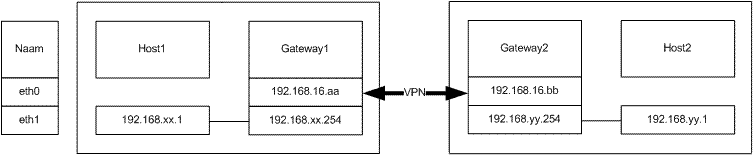
\includegraphics[width=\textwidth]{ipsec}
	\caption{IPSec configuratie.}
	\label{fig:ipsec}
\end{figure}

In deze opstelling blijven enkel de twee gateways verbonden met het bestaande netwerk via de lan0 interface, en zijn de IP-adressen 192.168.16.(aa bb) de originele IP-adressen van je toestel. De VPN-verbinding op de figuur loopt dus over het bestaande 192.168.16/24 netwerk.

Maak op de gateways gebruik van wireshark om alle inkomende en/of uitgaande IP-pakketten te bekijken. Ga steeds na of de IP-pakketten over de juiste headers beschikken (ESP en/of AH) en of de payload al dan niet werd geëncrypteerd. 

\section{Opgave}


\begin{enumerate}
	\textbf {\item Voorzie een veilige IPSec-verbinding tussen de twee clientcomputers. Test eerst uit met ESP zonder AH, daarna met AH zonder ESP.
	Voor deze vraag maak je nog geen gebruik van een combinatie van beide of van tunneling.}

 	\hrulefill
 	
 	Verkorte notatie: x = 192.168.70.1 en y = 192.168.76.1
 	
 	Voer het commando \texttt{setkey -f bestandsnaam} uit, met \textbf{bestandsnaam} de naam van het configuratiebestand waarin volgende instellingen komen.
 	
 	\begin{itemize}
 		\item \textbf{ESP configuratie.}
 		\begin{itemize}
 			\item hilbert
			\begin{lstlisting}
spdflush; -> zit in elk bestand
flush; -> zit in elk bestand
add y x esp 0x01 -m transport -E des-cbc "01234567";
add x y esp 0x02 -m transport -E des-cbc "01234567";
spdadd y x any -P out ipsec esp/transport//require;
spdadd x y any -P in ipsec esp/transport//require;
 			\end{lstlisting}
 			
 			\item fermat
 			
 			\begin{lstlisting}
add y x esp 0x01 -m transport -E des-cbc "01234567";
add x y esp 0x02 -m transport -E des-cbc "01234567";
spdadd x y any -P out ipsec esp/transport//require;
spdadd y x any -P in ipsec esp/transport//require;
 			\end{lstlisting}
 		\end{itemize}
 		
 		
 		
 		\item \textbf{AH configuratie.}
 		 		\begin{itemize}
 			\item hilbert
 			\begin{lstlisting}
add y x esp 0x01 -m transport -A hmac-md5 "0123456789ABCDEF";
add x y esp 0x02 -m transport -A hmac-md5 "0123456789ABCDEF";
spdadd y x any -P out ipsec ah/transport//require;
spdadd x y any -P in ipsec ah/transport//require;
 			\end{lstlisting}
 			
 			\item fermat
 			
 			\begin{lstlisting}
add y x esp 0x01 -m transport -A hmac-md5 "0123456789ABCDEF";
add x y esp 0x02 -m transport -A hmac-md5 "0123456789ABCDEF";
spdadd x y any -P out ipsec ah/transport//require;
spdadd y x any -P in ipsec ah/transport//require;
 			\end{lstlisting}
 		\end{itemize}
 	\end{itemize}
 	

 		
	\textbf {\item  Voortbouwend op de vorige vraag test je nu uit of je het verkeer tussen de clients kan encrypteren en bovendien ook kunt voorzien van de nodige authenticatie. Opnieuw wordt er geen tunneling gebruikt.
	Om dit te realiseren zijn er twee mogelijkheden, eerst encrypteren en dan authenticeren of omgekeerd. Test beide mogelijkheden uit en ga telkens na of er tussen de clients nog communicatie mogelijk is. Wanneer dit niet het geval is, maak je een schets om aan te tonen dat de uitgeteste configuratie niet kan werken.}
	
	\hrulefill
	
	De combinatie waarbij AH eerst gebruikt wordt is onmogelijk. AH zal eerst het bericht authenticeren op basis van de IP header. ESP zal deze IP header overschrijven, waardoor het onmogelijk is om de authenticatie te bevestigen. Eerst ESP, gevolgd door AH zal werken. 
	
	\begin{itemize}
		\item hilbert 
			\begin{lstlisting}
add y x esp 0x01 -m transport -E des-cbc "01234567";
add y x esp 0x02 -m transport -A hmac-md5 "0123456789ABCDEF";.
spdadd y x any -P out ipsec esp/transport//require ah/transport//require;
spdadd x y any -P in ipsec esp/transport//require ah/transport//require;
			\end{lstlisting}
		\item fermat 
			\begin{lstlisting}
add y x esp 0x01 -m transport -E des-cbc "01234567";
add y x esp 0x012 -m transport -A hmac-md5 "0123456789ABCDEF";.
spdadd x y any -P out ipsec esp/transport//require ah/transport//require;
spdadd y x any -P in ipsec esp/transport//require ah/transport//require;
			\end{lstlisting}
	\end{itemize}
	

	
	
	
	
	\textbf {\item  Op de clientcomputers behoud je het authenticatiegedeelte in transportmode. Het is dus niet nodig om het verkeer tussen beide clients te encrypteren.
	Tussen de gateways voorzie je nu bovendien een IPSec-tunnel. Test eerst uit met een AH-tunnel, daarna met een ESP-tunnel. Maak bij iedere opstelling een schets die aantoont of de gevraagde configuratie mogelijk is.}

\hrulefill

Extra notatie: a = 192.168.70.254 en b = 192.168.76.254
	
	\textbf {\item  Net zoals bij de vorige vraag zet je tussen de beide gateways een ESP-tunnel op. Aanvullend zorg je ervoor dat er tussen beide gateways authenticatie gebeurt in transportmode.
	Beide clients maken nog steeds gebruik van AH in transportmode. Test grondig uit en maak opnieuw de nodige schetsen.}
	
	\textbf {\item  Herneem de vorige vraag maar gebruik nu de racoon-daemon voor het aanmaken van de SA's op de clients en op de gateways. Om niet vanaf nul te moeten vertrekken kan je gebruikmaken van dit configuratiebestand. Vergeet niet om het bestand /etc/racoon/psk.txt aan te vullen zodat beide eindpunten over dezelfde sleutel beschikken.
	Ter info: wanneer er geen verkeer optreedt tussen de eindpunten, worden er door racoon geen nieuwe SA's aangemaakt! Je doet er dus goed aan om steeds een console open te houden waar je een ping stuurt naar het andere eindpunt.}
	
	\textbf {\item  Tot slot kan je eens nagaan wat er gebeurt als je tussen de gateways een dubbele tunnel opzet (ESP en AH in tunnelmode). Test uit in welke mate de volgorde een rol speelt en maak opnieuw een schets om na te gaan of het gevraagde enerzijds mogelijk is en anderzijds zinvol is.}
\end{enumerate}


\chapter{PGP}
Dit labo voer je elk afzonderlijk uit op je eigen \textbf{virtuele machine}, dus niet in groep. Maak op je VM drie gewone gebruikers aan: \textit{pgp1, pgp2} en \textit{pgp3}. Alle vollgende opdrachten voer je uit als één van deze gebruikers.
\section{Sleutelbeheer}
	\begin{figure}[h]
	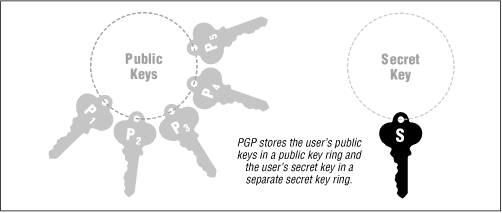
\includegraphics[width=\textwidth]{keyrings}
	\caption{Keyrings}
	\label{fig:keyrings}
\end{figure}
\subsection{Aanmaken sleutels}
\textbf{Maak voor gebruiker \textit{pgp1} drie sleutelparen aan (RSA and RSA, DSA en RSA). Voor gebruikers \textit{pgp2} en \textit{pgp3} maak je telkens twee sleutelparen aan; een RSA and RSA sleutelpaar en een DSA-sleutelpaar. Zorg er voor dat elke sleutel een verschillend ID heeft die de naam van de gebruiker bevat alsook de encryptiemethode. Kies een verschillende geldigheidsperiode voor de sleutels.}


	 Indien gpg nog niet geïnstalleerd is :
	$$\texttt{yum install gpg}$$
	Het kan zijn dat hij de mirrors niet kan resolven, clear de cache dan:
	$$\texttt{yum clean all}$$
	Installeer ook de rng-tools om entropy te genereren:
	$$\texttt{yum install rng-tools}$$
	In de virtual machine kan je nieuwe terminals openen via CTRL + $\vert$ F1 $\vert$ F2 $\vert$ F3 $\vert$ ... $\vert$ F7. Log in op deze verschillende terminals als de drie gebruiker accounts. Behou ook nog een terminal voor de root gebruiker (CTRL + F1 voor root bijvoorbeeld). Run het commando rng-tools in de voorgrond, zodat het random activiteit zal blijven genereren, dit is nodig bij het genereren van sleutels:
	$$\texttt{/usr/sbin/rngd -f -r /dev/urandom}$$
	
	Een sleutel genereren kan met 
	$$\texttt{gpg --gen-key}$$
	Als \textit{pgp1} doe je dit drie keer, telkens met een verschillend algoritme. Als \textit{pgp2} en \textit{pgp3} twee keer: eens met DSA en dan met RSA. 
\begin{itemize}
	\item \textbf{Waarvoor dient de passphrase?} De passphrase dient om de private sleutel te beschermen. Sommige acties op sleutels vereisen ook deze passphrase.
	\item \textbf{Waarom wordt er bij het aanmaken van een sleutel soms naar extra toetsaanslagen gevraagd en soms ook niet?} GPG maakt gebruik van activiteiten zoals toestaanslagen en muisbewegingen (systeemactiviteiten) om entropy te genereren. Gelukkig kan dit vermeden worden door \textit{rngd} te gebruiken.
	\item \textbf{Wat is het verschil tussen "RSA and RSA" en "DSA and Elgamal"?}
\subsection{Exporteren en uitwisselen sleutels}
\textbf{Exporteer al je publieke sleutels naar meerdere bestanden die je aan andere gebruikers kan aanbieden. Exporteer deze in 2 verschillende formaten, waarvan er één geschikt is voor transport via e-mail of publicatie op een webserver.}

Gebruik het volgende commando om één enkele sleutel te exporteren. De variabele \texttt{UNIEKE\_NAAM} bevat een identificatie van de sleutel (bv op basis van Real Name en Comment, of gewoon het ID van de sleutel). 
$$\texttt{gpg --export UNIEKE\_NAAM --output \textasciitilde/outputnaam}$$
Voor leesbare exports gebruik je de \texttt{--armor} optie:
$$\texttt{gpg --armor --export UNIEKE\_NAAM --output \textasciitilde/outputnaam}$$
Het is ook mogelijk om alle sleutels direct te exporten, door geen argument mee te geven aan \texttt{--export}:
$$\texttt{gpg --export --output \textasciitilde/outputnaam}$$
\textbf{Wat is het formaat van deze bestanden?} Zonder de \texttt{--armor} optie hebben de exportbestanden een binair formaat. Deze bestanden uitprinten op een terminal heeft dan ook geen nut. Met de \texttt{--armor} optie ziet het er bijvoorbeeld als volgt uit (ingekort):
\begin{lstlisting}
-----BEGIN PGP PUBLIC KEY BLOCK-----
Version: GnuPG v1.2.1 (GNU/Linux)
Comment: For info see http://www.gnupg.org

mQGiBDkHP3URBACkWGsYh43pkXU9wj/X1G67K8/DSrl85r7dNtHNfLL/ewil10k2
q8saWJn26QZPsDVqdUJMOdHfJ6kQTAt9NzQbgcVrxLYNfgeBsvkHF/POtnYcZRgL
=BMEc
-----END PGP PUBLIC KEY BLOCK-----
\end{lstlisting}

\textbf{Wissel deze bestanden uit met de andere gebruikers (bv. door ze in een gedeelde directory te plaatsen). We gaan er op dit ogenblik van uit dat sleutels die op deze manier zijn verkregen, volledig te vertrouwen zijn.} 

De eenvoudigste manier is om als root gebruiker de bestanden te kopieëren naar de root folder van elke gebruiker (gebruik hiervoor de terminal die voor de root gebruiker beschikbaar is).
$$\texttt{cp /home/pgp1/exportbestand /home/pgp2/exportbestand\_pgp1}$$
\end{itemize}

\subsection{Toevoegen sleutels}
\textbf{Voeg voor elke gebruiker de verkregen publieke sleutels toe aan zijn publieke sleutelhanger. Verifieer of ze wel zijn opgenomen.}

Een sleutel importeren kan met 
$$\texttt{gpg --import bestandsnaam}$$
Dit commando zal ook specificeren hoeveel publieke sleutels er zijn toegevoegd. Om een lijst van alle sleutels op te vragen gebruik je
$$\texttt{gpg --list-key}$$

\textbf{Verwijder één van de sleutels uit de sleutelhanger. Controleer en voeg de sleutel nadien weer toe.}

Een sleutel verwijderen kan met 
$$\texttt{gpg --delete-key sleutelID}$$

\subsection{Wijzigen sleutels}
\textbf{Wijzig één van de sleutels: verander de passeerzin.}
Een sleutel wijzigen kan met
$$\texttt{gpg --edit-key sleutelID}$$
Na het uitvoeren van dit commando zit je in een menu. Met \textit{help} kan je alle mogelijke opties ophalen. Een passphrase veranderen kan met \textit{passwd}.

\subsection{Vertrouwen sleutels}
\begin{itemize}
	\item \textbf{Controleer de sleutels en de handtekeningen die er bij horen.}
	\item \textbf{Verifieer de fingerprint van de sleutels bij de verschillende gebruikers.}
	
	Gebruik \texttt{gpg --verify sleutelID}
	\item \textbf{Zorg er voor dat al de sleutels in de sleutelhangers volledig vertrouwd worden, indien dit nog niet het geval zou zijn.}
	
	Een sleutel vertrouwen kan terug met \texttt{gpg --edit-key sleutelID}.
	In het menu gebruik je nu \texttt{trust}, en geef je ultimate trust aan elke sleutel. Hiervoor moet dus elke keer het gpg commando met de \texttt{--edit-key} optie uitgevoerd worden voor elke sleutel.
	\item \textbf{Teken voor elke gebruiker de eigen sleutels en die van de andere gebruikers van wie de sleutel vertrouwd wordt.}
	
	Gebruik hiervoor de \texttt{sign} optie in de \texttt{--edit-key} menu.
\end{itemize}

\section{Encrypteren en decrypteren van bestanden}
\begin{figure}[h]
	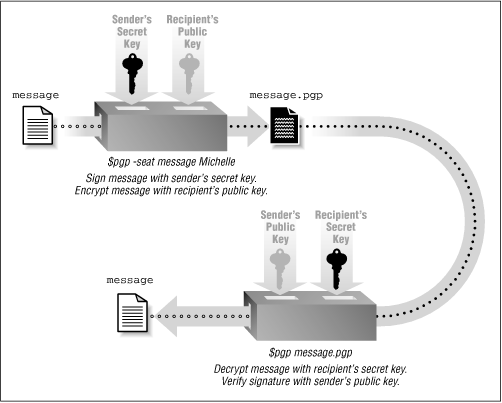
\includegraphics[width=\textwidth]{encrypting}
	\caption{Encryptie.}
	\label{fig:encrypting}
\end{figure}
\subsection{Lokaal encrypteren en decrypteren}
\textbf{Maak als gebruiker \textit{pgp1} vijf korte tekstbestanden aan om ze nadien aan de andere gebruikers over te maken. Encrypteer deze bestanden als volgt: }
\begin{enumerate}
	\item \textbf{het eerste bestand encrypteer je door middel van conventionele encryptie op twee manieren:
		de eerste keer met het default algoritme,
		de tweede keer geef je zelf het algoritme op (bv. AES256). }
	Het default algoritme is CAST5. Het volgende commando zal een bestand encrypteren met dit algoritme:
	$$\texttt{gpg --encrypt bestand1}$$
	Er zal een prompt komen voor User IDs, laat dit voorlopig leeg. Het uitvoerbestand zal \texttt{bestand1.gpg} zijn. Dit zullen ook de bestanden zijn die moeten verzonden worden over een netwerk naar de begunstigde.
	
	
	Zelf aan algoritme meegeven kan met de \texttt{--cipher-algo} optie:
	$$\texttt{gpg --encrypt --cipher-algo AES256 bestand1}$$
	
	\item \textbf{het tweede bestand encrypteer je zodat alleen gebruiker pgp2 het bestand kan decrypteren.}
	
	Hier wordt ervan uitgegaan dat de naam van de sleutels van de gebruiker pgp2, zelf ook de string "pgp2" bevatten.
	$$\texttt{gpg --encrypt --recipient pgp2 bestand2}$$
	
	\item \textbf{het derde bestand encrypteer je zodat dit door gebruikers pgp2 en pgp3 kan ontcijferd en gelezen worden. Zorg dat de encryptie met een ander dan het default algoritme gebeurt.}
	$$\texttt{gpg --encrypt --cipher-algo AES256 bestand3}$$
	Vul nu in de prompt twee User IDs in, namelijk die van pgpp2 en pgp3 (op aparte lijnen).
	
	\item \textbf{het vierde bestand encrypteer je zodat gebruiker pgp2 hem niet zonder meer kan opslaan op zijn vaste schijf.}
	
	???
	
	\item \textbf{het vijfde bestand encrypteer je conventioneel maar het resultaat is in radix64.}
\end{enumerate}

\textbf{Veeg de originele plaintextbestanden uit. Probeer nu de plaintext te herstellen uitgaande van de ciphertext van elk bestand. Controleer wat er al dan niet nog kan gebeuren}

\subsection{Remote decrypteren}
\textbf{Wissel al de geëncrypteerde bestanden uit met de gebruikers pgp2 en pgp3. Decrypteer alle ontvangen bestanden. Beschrijf in elk van de gevallen wat er gebeurt.}
Een bestand decrypteren kan met:
$$\texttt{gpg --decrypt bestandsnaam}$$
Indien dit bestand bedoeld was voor de huidige gebruiker, dan zal hij deze kunnen decrypteren, en zal de inhoud van het bestand naar de console geschreven worden. Is dit niet zo zal er een foutmelding komen dat de juiste sleutel niet beschikbaar is.

\section{Sleutelbeheer}


\end{document}

